\begin{exercise}{trigonometrie.winkelgroessen}{Winkelgrößen}
  \ifproblem\problem\par
    Die abgebildeten Figuren bestehen aus zwei aneinander gelegten Quadraten.
    Die markierten Punkte sind jeweils Seitenmittelpunkte. Berechne die
    Winkelgrößen.
    \begin{center}
      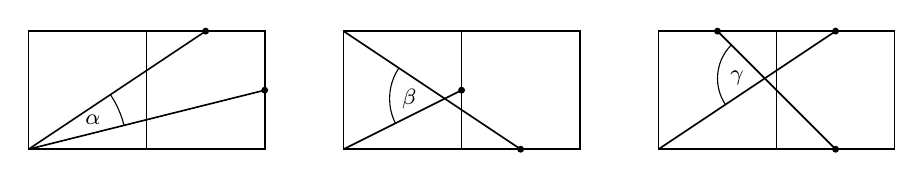
\begin{tikzpicture}
        \begin{scope}
          \coordinate (A) at (0.00, 0.00);
          \coordinate (B) at (3.00, 0.75);
          \coordinate (C) at (2.25, 1.50);
          % Rechteck
          \draw[line width=0.6pt] (0.0, 0.0) rectangle (3.0, 1.5);
          % Mittellinie
          \draw[line width=0.6pt] (1.5, 0.0) -- (1.5, 1.5);
          % Schenkel
          \draw[line width=0.6pt] (A) -- (B);
          \draw[line width=0.6pt] (A) -- (C);
          % Seitenmittelpunkte
          \fill (B) circle (1.25pt);
          \fill (C) circle (1.25pt);
          % Winkel
          \begin{scope}
            \clip (A) -- (B) -- (C) -- cycle;
            \draw[line width=0.4pt] (A) circle (1.25cm);
            \node[shift=(24.5:9mm)] at (A) {{\footnotesize$\alpha$}};
          \end{scope}
        \end{scope}
        \begin{scope}[xshift=4cm]
          \coordinate (A) at (0.00, 0.00);
          \coordinate (B) at (1.50, 0.75);
          \coordinate (C) at (0.00, 1.50);
          \coordinate (D) at (2.25, 0.00);
          \coordinate (S) at (intersection of A--B and C--D);
          % Rechteck
          \draw[line width=0.6pt] (0.0, 0.0) rectangle (3.0, 1.5);
          % Mittellinie
          \draw[line width=0.6pt] (1.5, 0.0) -- (1.5, 1.5);
          % Schenkel
          \draw[line width=0.6pt] (A) -- (B);
          \draw[line width=0.6pt] (C) -- (D);
          % Seitenmittelpunkte
          \fill (B) circle (1.25pt);
          \fill (D) circle (1.25pt);
          % Winkel
          \begin{scope}
            \clip (A) -- (S) -- (C) -- cycle;
            \draw[line width=0.4pt] (S) circle (7mm);
            \node[shift=(180:4.5mm)] at (S) {{\footnotesize$\beta$}};
          \end{scope}
        \end{scope}
        \begin{scope}[xshift=8cm]
          \coordinate (A) at (0.00, 0.00);
          \coordinate (B) at (2.25, 1.50);
          \coordinate (C) at (0.75, 1.50);
          \coordinate (D) at (2.25, 0.00);
          \coordinate (S) at (intersection of A--B and C--D);
          % Rechteck
          \draw[line width=0.6pt] (0.0, 0.0) rectangle (3.0, 1.5);
          % Mittellinie
          \draw[line width=0.6pt] (1.5, 0.0) -- (1.5, 1.5);
          % Schenkel
          \draw[line width=0.6pt] (A) -- (B);
          \draw[line width=0.6pt] (C) -- (D);
          % Seitenmittelpunkte
          \fill (B) circle (1.25pt);
          \fill (C) circle (1.25pt);
          \fill (D) circle (1.25pt);
          % Winkel
          \begin{scope}
            \clip (A) -- (S) -- (C) -- cycle;
            \draw[line width=0.4pt] (S) circle (6mm);
            \node[shift=(180:3.5mm)] at (S) {{\footnotesize$\gamma$}};
          \end{scope}
        \end{scope}
      \end{tikzpicture}
    \end{center}
  \fi
  %\ifoutline\outline\par
  %\fi
  %\ifoutcome\outcome\par
  %\fi
\end{exercise}
